% TODO: lacks some narrative flow between sections

% TODO: end would benefit from "summary section" (not sure what that means) that
% reflects on high level trends in the literature, building into a proposed
% strategy and thus flowing into the methodology.
This work builds upon much prior research into powerful deep generative
models, self-supervised methods, and efficient
transformer architectures. We briefly cover relevant prior work into deep
generative models in general in \S\ref{subsec:agm}-\ref{subsec:vqmodelling}, a
particular \acrshort{nar} generative model we wish to build upon in
\S\ref{subsec:sundae}, and a recent and highly effective development into a
efficient transformer architecture in \S\ref{subsec:hourglass}. For a full
review on generative modelling we direct the reader to
\citet{bondtaylor2021review}, and for further details on \gls{sundae} and
hourglass transformers we direct the reader to \citet{savinov2022stepunrolled}
and \citet{nawrot2021hierarchical} respectively.

\begin{figure}[ht!]
    \centering
    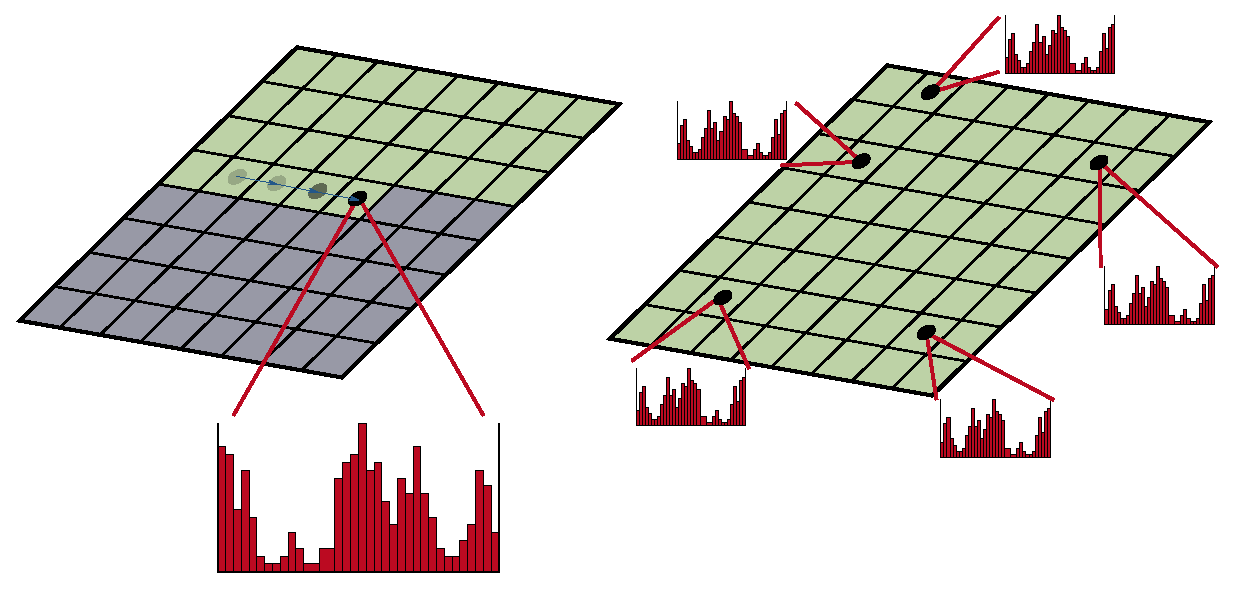
\includegraphics[width=\textwidth]{figures/AR-NAR.pdf}
    \caption{
        \textbf{Left:} Visualization of \acrfull{ar} sampling. \gls{ar} sampling
        proceeds one item at a time, resulting in the number of sampling steps
        being equal to the dimensionality of the input. For each prediction, a
        probability distribution over possible tokens is predicted and then
        sampled from. Each prediction can only make use of past context --
        indicated as a green position -- so not to violate the autoregressive
        property.
        \textbf{Right:} Visualization of \acrfull{nar} sampling. \gls{nar}
        sampling can sample an arbitrary number of items in parallel, including
        ones previously sampled, allowing for self-correction. It can freely use
        all context available to it, allowing for flexible inpainting and
        potentially better predictions.
    }
\end{figure}

\subsection{Autoregressive Generative Models}
\label{subsec:agm}
One major deep generative model family is \acrfull{ar} models, characterised by
a training and inference process based on the probabilistic chain rule. During
training, they directly aim to maximise the likelihood of the data they are
trained on, which leads to excellent mode coverage. Prior work using these
methods resulted in impressive results in terms of both sample quality and
diversity, but are ultimately unwieldy for use in real world applications due to
their slow sampling speed.

The slow sampling speed is due to their sequential nature, defined by the chain
rule of probability. Given an input $\image = \{ \pixel{1}, \pixel{2}, \dots,
\pixel{n} \}$, an \gls{ar} model $p_\theta(\cdot)$ can generates new
samples sequentially:
\begin{equation}\label{eq:ar}
    p_\theta(\image) = p_\theta(\pixel{1}, \dots, \pixel{n}) =
    \prod\limits^{n}_{i=1} p_\theta(\pixel{i} \vert \pixel{1}, \dots, \pixel{i-1})
\end{equation}
meaning that the number of sampling steps is equal to the size of the
decomposition of $\image$, making this slow for large inputs.

For certain tasks, the ordering of the decomposition of $\image$ is obvious, for
example on text or speech. For images this is less obvious, however typically a
raster scan ordering is used. Certain \gls{ar} models are order-agnostic,
allow for arbitrary ordering to be used during training and inference.

One class of \gls{ar} models are \glspl{rnn} which are an early example of using
neural networks to model sequential data, such as text, audio, time-series data,
or even vector handwriting strokes. Though they can be used as purely
classification or regression models, they are also suited for use as generative
models by modelling the relationship shown in Equation~\ref{eq:ar}. They do
suffer from a number of issues, most notably vanishing
gradients~\cite{pascanu2012rnn} and inability to model long-range relationships
between items in the input. \Glspl{lstm}~\cite{hoch1997lstm} improved upon them
further by introducing dedicated memory units, allowing for the modelling of
longer range relationships. Later \glspl{gru}~\cite{cho2014gru} simplified the
architecture whilst still retaining good performance. With the advent of
transformer architectures~\cite{vaswani2017attention}, modelling even longer
relationships became possible, even at a full-document level. It also intro cued
the capability to train on all sequence elements in parallel through the use of
causal masking, therefore not violating the autoregressive property.

Applying \gls{ar} models to images followed a similar trend.
PixelRNN~\cite{oord2016pixelrnn} used two-dimensional recurrent layers and
residual connections to model the distribution of raw pixel values. The same
paper also introduced PixelCNN, which it claims had worse performance but were
faster to train. These were extended to allow for conditional generation
in~\cite{oord2016pixelcnn}. Later work augmented PixelCNN with self-attention
mechanism, forming PixelSnail~\cite{chen2017snail}, which can therefore model
longer relationships than a fully convolutional or recurrent architecture. Image
Transformer~\cite{parmar2018image} later applied transformer architectures to
the same task through an effective but altogether conceptually simple approach.

\subsection{Non-autoregressive Generative Models}
\label{subsec:nagm}
\Acrfull{nar} generative models include \glspl{gan}, \glspl{sbm} and
\glspl{ddpm}, flow-based models, \glspl{ebm}, and implicit models. Though the
number of sampling steps is now independent of the data dimensionality (as we no
longer use the chain rule of probability to sample) the actual number of steps
varies greatly: from single-step generation in \glspl{gan} to potentially many
thousands in the original diffusion model literature.

% TODO: discuss briefly each from of NAR model and its strengths/weaknesses
% - [X] GAN
% - [X] Variational autoencoders
% - [X] SBM / DDPM
% - [X] Normalizing flows

Perhaps the most infamous class of \gls{nar} generative model -- or perhaps
generative model overall -- are \acrfullpl{gan}~\cite{goodfellow2014gan}. These
typically consist of two components: a generator that create images from some
latent variable (in the most basic case just random noise), and a discriminator
that tries to distinguish images from the dataset from images generated by the
generator network~\cite{goodfellow2014gan}. They are known for high-fidelity
samples, fast sampling, unstable training, and tendency to collapse onto certain
modes of the underlying distribution due to not optimising directly for
likelihood. This is reflected in its relatively low-diversity samples.
Nonetheless, the quality of the samples has made them a popular choice in a
variety of applications, including unconditional and conditional
generation~\cite{tero2018stylegan,andrew2018biggan} image, audio
synthesis~\cite{liu2020audiogan}, style transfer~\cite{zhu2017cyclegan}. They
can even be applied to discrete data~\cite{autume2019scratchgan}, but are less
effective on such domains due to the non-differentiability of discrete samples.

Another class of generative model are \acrfullpl{vae}~\cite{kingma2013vae} which
allow for sampling in a single forward pass like \glspl{gan}, but are trained to
directly maximise likelihood. Specifically, \glspl{vae} map inputs to latent
variables that follow some easy to sample from, but still sufficiently complex,
prior distribution. A common choice is a multivariate Gaussian with diagonal
covariance~\cite{kingma2013vae}. A decoder network maps these latent codes back
to the data distribution. Although this approach is successful on small
datasets, on more complex datasets the samples and reconstructions tend to
become blurry, suggesting a simple prior is unable to perfectly fit the
distribution. Later work extended \glspl{vae} to be hierarchical, having
multiple Gaussian priors~\cite{arash2020nvae,child2020vqvae} which were found to
outperform purely autoregressive models.

Normalizing flows are another class of generative model that allows for exact
likelihood calculation. They consist of many invertible layers that gradually
transform samples from a known prior distribution into samples from the data
distribution. Each transformation must satisfy two properties: being invertible
and having an easy to compute Jacobian (allowing easy rescaling). This makes the
architecture quite restrictive, making them less parameter efficient. They also
typically must operate at the same dimensionality for each layer, making the
training of deep networks difficult.

Two paradigms that are gaining a lot of interest in recent times are
\acrfullpl{ddpm}~\cite{ho2020ddpm} and \acrfullpl{sbm}~\cite{song2019sbm}. Both
are variants of \glspl{ebm}, with the former learning to estimate the noise at
various levels (which can be used to gradually move from noise to data), and the
latter trained to remove noise, given corrupted samples from a gradually
corrupting forward process. Again, this can be used to move from pure noise back
to data. Both are slow to sample from, but produce high quality samples that
rival those of \glspl{gan}~\cite{dhariwal2021ddpm} whilst not suffering from
mode collapse. The slow sampling speed can be remedied using a variety of
techniques, such as operating on a smaller latent
space~\cite{vahdat2021sbmlatent}, devising more
efficient SDE solvers~\cite{martineau2021fast}, or by diffusing the
``velocities'', thus simplifying the denoising task~\cite{dockhorn2021langevin}.
Unlike GANs, both models can also operate on discrete data, such as by first
projecting discrete data into a continuous latent
space~\cite{vahdat2021sbmlatent} or with a dedicated discrete diffusion
framework~\cite{austin2021structured}, the latter of which bridges the gap
between diffusion, autoregressive, and mask-based representation models.

%Removing the causal constraints also allows for bidirectional context during
%sampling and flexible inpainting patterns, rather than being limited to
%left-to-right inpainting in autoregressive models.

\subsection{Vector Quantized Image Modelling}
\label{subsec:vqmodelling}
% TODO: maybe add a nice table comparing all the methods
% TODO discuss: VQ modelling in connection with generative modelling. 
Learning useful representations, also known as latent codes, in an unsupervised
manner is a key challenge in machine learning. Historically, these
representations have been in a continuous form, but in more recent literature
they are often discrete. An early example of this is
\gls{vqvae}~\cite{oord2017vqvae}, a variant on \gls{vae} representation models.
A \gls{vqvae} has three main components: an encoder network, a codebook, and a
decoder. The encoder network outputs a compressed representation of the input,
and the codebook $\vqganCodebook$ quantizes these representations, outputting a
discretized representation of indices from $1$ to the codebook size
$\vqganNbLatents$. Each index $i$ maps to one of the codebook embeddings $e_i$.
The decoder then maps the quantized embeddings back to the original signal,
training it in tandem to reconstruct the input signal and to minimize additional
codebook loss terms~\cite{oord2017vqvae}. Once a trained \gls{vqvae} model has
been produced, a powerful auxiliary generative model can be trained to generate
these discrete latent representations and then the decoder can produce the final
sample. In the original work on \gls{vqvae}, they use a PixelCNN model to
generate the discrete latent codes~\cite{oord2017vqvae}, though any generative
model on discrete data can be used.

\begin{figure}[ht!]
    \centering
    %\includesvg[width=\textwidth]{figures/vq.svg}
    \includegraphics[width=\textwidth]{figures/vq.pdf}
    \caption{
        Visualisation of a vector-quantization image model. An encoder model
        first extracts continuous embeddings from the source image. Vector
        quantization is then used to map each continuous embedding to the
        closest entry in the codebook. A decoder model takes the discretized
        embeddings and attempts to reconstruct the original image. We can
        produce a dataset of latent embeddings from a source image dataset 
        by sampling $\image \sim \imageDataset$ and appending the resulting
        discretized embeddings $\latent$ to a dataset $\latentDataset$.
    }
\end{figure}

Later approaches extended \gls{vqvae} to multiple distinct codebooks in
\acrshort{vqvae}-2~\cite{razavi2019generating}. Though theoretically it can be
extended to any number of codebooks, they performed experiments on a two-level
and three-level model, applying the latter to $1024 \times 1024$ images. They
then sampled the resulting combined discrete codes use
PixelSnail~\cite{chen2017snail}, each code conditioned on all previous levels in
the hierarchy. Though faster to sample than applying a generative directly to
pixels, at such a resolution and with multiple levels to sample, sampling times
were still slow.

Aside from sampling autoregressively, a reason for the slow sampling speed was
the large spatial resolution of the discrete codes. Albeit smaller than the
original signal, \gls{vqvae} is limited in how much it can compress the signal
via a simple reconstruction objective before it loses too much perceptual
quality due to the rate-distortion trade-off. For example, the original
\gls{vqvae} only has a downsampling rate of
$\vqganDownsample=4$~\cite{oord2017vqvae} and \gls{vqvae}-2 has a rate of
top-level rate of $\vqganDownsample=32$ but requires a total of three discrete
latent codes in order to achieve this~\cite{razavi2019generating}. By
introducing perceptual and adversarial loss terms,
\gls{vqgan}~\cite{esser2021taming} is able to achieve compression rates of
$\vqganDownsample=16 \sim 32$ with only a single discrete latent representation
whilst retaining high quality reconstructions~\cite{esser2021taming}. The
greater weighting on perceptual and adversarial loss does mean, however, that
\gls{vqgan} does sometimes edit its reconstructions, rather than attempt to
preserve all details perfectly like when using a simple reconstruction loss
alone. Later, improvements such as differential data
augmentation~\cite{bondtaylor2021unleashing}, codebook improvements, and a
transformer-based architecture~\cite{yu2021vqgan} improved reconstruction
quality further.

Originally designed for audio compression~\cite{zeghidour2021soundstream},
Residual \gls{vq} proposes the use of multiple codebooks to recursively quantize
and refine the residual of an input signal. This produces multiple discrete
representations, which can later be reconstructed by the decoder to decompress
the waveform. Additionally, individual codebooks can be dropped out, allowing
for variable bit-rates~\cite{zeghidour2021soundstream}. Concurrently to this
work, \citet{lee2022rqvae} used residual \gls{vq} to represent images with a
compression ratio of $\vqganDownsample=32$ and then trained a transformer model
to autoregressively predict the stack of discrete tokens at a given spatial
location, allowing for fast sampling despite actually having multiple levels of
discrete latent representations\cite{lee2022rqvae}.

\begin{table}[ht]
    \centering
    \begin{tabular}{|c|c|c|c|c|c|}
        \hline
        \textbf{Model} & \textbf{Input Size} & \textbf{Latent Shape} & \textbf{Codebook Size} & \textbf{FID/val} & \textbf{FID/train} \\
        \hline
        VQ-VAE & $128 \times 128$ & $32 \times 32$ & $512$ & -- & -- \\
        \hline
        VQ-VAE-2 & $256 \times 256$ & $64 \times 64$ \& $32 \times 32$ & $512$ & --& $\sim 10$ \\
                 & $1024 \times 1024$ & $128 \times 128$ \& $64 \times 64$ \& $32 \times 32$ & $512$ & -- & -- \\
        \hline
        DALLE & $256 \times 256$ & $32 \times 32$ & $8192$ & $32.01$ & $33.88$ \\
        \hline
        VQ-GAN & $256 \times 256$ & $16 \times 16$ & $1024$ & $7.94$ & $10.54$ \\
        & $256 \times 256$ & $16 \times 16$ & $16384$ & $4.98$ & $7.41$ \\
        & $256 \times 256$ & $32 \times 32$ & $8192$ & $1.49$ & $3.24$ \\
        & $256 \times 256$ & $64 \times 64$ \& $32 \times 32$ & $8192$ & $1.45$ & $2.78$ \\
        \hline
        RVQ-VAE & $256 \times 256$ & $8 \times 8 \times 2$ & $16384$ & -- & $10.77$ \\
        & $256 \times 256$ & $8 \times 8 \times 4$ & $16384$ & -- & $3.20$ \\
        & $256 \times 256$ & $8 \times 8 \times 8$ & $16384$ & -- & $2.69$ \\
        & $256 \times 256$ & $8 \times 8 \times 16$ & $16384$ & -- & $1.83$ \\
        \hline
    \end{tabular}
    \caption[Table]{Summary of various \acrfull{vq} methods. The trend with
    \gls{vq} image models is increasing compression rates $\vqganDownsample$ and
    codebook sizes. However, to obtain these compression rates techniques such
    as perceptual and adversarial losses must be used.}
\end{table}

A typical strategy for selecting which codebook vector $e_i$ to map to a
particular input is to compute the Euclidean distance between a given continuous
input and the codebook centroid, and then pick the
$\arg\min$~\cite{oord2017vqvae}. This is denoted the $k$-means strategy. This
strategy does result in a phenomena known as codebook collapse, where certain
codebook vectors never get used, harming the downstream reconstruction quality.
An alternative method is to use the Gumbel-Softmax~\cite{jang2016gumbel} to
select codebook vectors, which typically increases codebook utilisation but
often leads to worse reconstruction quality~\cite{bondtaylor2021unleashing}.

The issue of codebook collapse is quite significant and there have been a number
of attempts to remediate it. \cite{yu2021vqgan} found that a lower codeword
dimension and codeword normalization improved utilisation.
\cite{zeghidour2021soundstream} proposed setting a threshold for ``stale'' codes,
and reinitialisating them to a random vector from the current batch when they
fall below this threshold. \cite{lee2022rqvae} proposed the sharing of a single
codebook across many quantizers and additionally stochastically sampled the
codes as a function of their distance to the centroid, rather than always taking
the $\arg\min$.

All these previous approaches use \gls{vq} models to enhance existing
\gls{ar} models, primarily to improve their sampling speed by reducing the
spatial dimension we are operating over. Few work directly addresses the
discrete prior model itself. Discrete diffusion
models~\cite{austin2021structured} are \gls{nar} approach to generate discrete
data. This was applied to \gls{vqgan} latents in
\citet{bondtaylor2021unleashing}, allowing for fast sampling, flexible
inpainting, and high fidelity outputs.

\subsection{Step-unrolled Denoising Autoencoder}
\label{subsec:sundae}
One recent \gls{nar} model is \gls{sundae}~\cite{savinov2022stepunrolled} which
was evaluated on three language modelling tasks: unconditional text-generation,
inpainting of Python code, and machine translation -- setting a new
state-of-the-art among \gls{nar} models for the machine translation
task~\cite{savinov2022stepunrolled}. It also demonstrates exceptionally fast
sampling, producing high quality samples in as few as 10 steps.

\gls{sundae} is trained using a denoising objective, akin to the
BERT denoising objective~\cite{wang2019bert} but with multiple denoising steps.
Given a uniform prior $p_0$ over some space $\latentSpace = \{1, \dots,
\vqganNbLatents\}^N$ where $N$ is the size of the space and $v$ is the
vocabulary size, consider the Markov process $\latent_t \sim \sundae(\cdot \vert
\latent_{t-1})$ where $\sundae$ is a neural network parameterised by
$\sundaeParameters$, then $\{\latent_t\}_t$ forms a Markov chain. This gives a
$t$-step transition function: \begin{equation}\label{eq:markov} p_t(\latent_t
    \vert \latent_0) = \sum\limits_{\latent_1, \dots, \latent_{t-1} \in
    \latentSpace} \prod\limits^t_{s=1} \sundae(\latent_s | \latent_{s-1})
\end{equation}\cite{savinov2022stepunrolled} and, given a constant number of
steps $\markovSteps$, our model distribution
$p_\markovSteps(\latent_\markovSteps \vert \latent_0)p_0(\latent_0)$ -- which is
clearly intractable.

Instead, they propose an \textit{unrolled denoising} training method that uses a
far lower $\markovSteps$ than is used for
sampling~\cite{savinov2022stepunrolled}. To compensate, they unroll the Markov
chain to start from corrupted data produced by a \textit{corruption
distribution} $\latent' \sim \corruptionDistribution(\cdot \vert \latent)$
rather than from the prior $p_0$ so the model encounters samples more akin to
those seen during the full unroll at sample time~\cite{savinov2022stepunrolled}.
Typically, $\markovSteps = 2$ during training, as a single step would be similar
to the training strategy of BERT~\cite{devlin2019bert} but would lead to worse
performance as seen in earlier work using BERT as a random field language
model~\cite{wang2019bert}.

The training objective of \gls{sundae} is simply the average of all reconstruction
losses $\lossFunction{1:T} = \frac{1}{T} \left(\lossFunction{1} + \dots +
\lossFunction{T} \right)$ of the chain after $t$ steps, which is shown to form
an upper bound on the actual negative
log-likelihood~\cite{savinov2022stepunrolled}. Taking more steps $\markovSteps$
leads to a minor improvement in performance, but considerably slows down
training time~\cite{savinov2022stepunrolled} and increases memory usage.

One advantage of this approach is that sampling starts from random tokens,
rather than a dedicated ``masking''
token~\cite{bondtaylor2021unleashing,austin2021structured}. Unmasking approaches
means that $\markovSteps \leq N$ as at minimum, one token is unmasked per step.
Additionally, it allows the model to be able to ``change its mind'' about
previously predicted positions during sampling, allowing it to make fine-grained
adjustments or fix accumulated errors.

\subsection{Hourglass Transformers}
\label{subsec:hourglass}

Vanilla transformers incur a hefty memory and time complexity of $O(L^2)$ for
each block~\cite{vaswani2017attention}. This is largely due to the multi-head
self-attention mechanism, as each input position must attend to every other.
Most research into efficient transformers focuses on improving the efficiency of
these attention mechanism, such as through sparse attention patterns or
approximations of attention.

Recent work however, is now focusing on making the overall architecture more
efficient. Funnel-Transformer~\cite{dai2020funneltransformer} progressively
downsamples the input sequence and hence reduces the computational cost of the
model. The saved \glspl{flop} can then be reassigned to create deeper or wider models
and thus outperform vanilla transformers given the same computational
budget~\cite{dai2020funneltransformer}. However, the final layer does not
operate at the same granularity as the input, making it unusable for tasks that
require this such as per-token classification or generative tasks. Hourglass
transformers~\cite{nawrot2021hierarchical} include both up- and down-sampling
mechanisms, resulting in a computational saving whilst still being
general-purpose models.
